%% abtex2-modelo-trabalho-academico.tex, v-1.9.2 laurocesar
%% Copyright 2012-2014 by abnTeX2 group at http://abntex2.googlecode.com/ 
%%
%% This work may be distributed and/or modified under the
%% conditions of the LaTeX Project Public License, either version 1.3
%% of this license or (at your option) any later version.
%% The latest version of this license is in
%%   http://www.latex-project.org/lppl.txt
%% and version 1.3 or later is part of all distributions of LaTeX
%% version 2005/12/01 or later.
%%
%% This work has the LPPL maintenance status `maintained'.
%% 
%% The Current Maintainer of this work is the abnTeX2 team, led
%% by Lauro César Araujo. Further information are available on 
%% http://abntex2.googlecode.com/
%%
%% This work consists of the files abntex2-modelo-trabalho-academico.tex,
%% abntex2-modelo-include-comandos and abntex2-modelo-references.bib
%%

% ------------------------------------------------------------------------
% ------------------------------------------------------------------------
% abnTeX2: Modelo de Trabalho Academico (tese de doutorado, dissertacao de
% mestrado e trabalhos monograficos em geral) em conformidade com 
% ABNT NBR 14724:2011: Informacao e documentacao - Trabalhos academicos -
% Apresentacao
% ------------------------------------------------------------------------
% ------------------------------------------------------------------------

\documentclass[
	% -- opções da classe memoir --
	12pt,				% tamanho da fonte
%	openright,			% capítulos começam em pág ímpar (insere página vazia caso preciso)
	oneside,			% para impressão em verso e anverso. Oposto a oneside
	a4paper,			% tamanho do papel. 
	% -- opções da classe abntex2 --
	%chapter=TITLE,		% títulos de capítulos convertidos em letras maiúsculas
	%section=TITLE,		% títulos de seções convertidos em letras maiúsculas
	%subsection=TITLE,	% títulos de subseções convertidos em letras maiúsculas
	%subsubsection=TITLE,% títulos de subsubseções convertidos em letras maiúsculas
	% -- opções do pacote babel --
	%english,			% idioma adicional para hifenização
	brazil
	%french,				% idioma adicional para hifenização
	%spanish,			% idioma adicional para hifenização
	%brazil				% o último idioma é o principal do documento
	%english
	]{abntex2}

% ---
% Pacotes básicos 
% ---
\usepackage{lmodern}			% Usa a fonte Latin Modern			
\usepackage[T1]{fontenc}		% Selecao de codigos de fonte.
\usepackage[utf8]{inputenc}		% Codificacao do documento (conversão automática dos acentos)
\usepackage{lastpage}			% Usado pela Ficha catalográfica
\usepackage{indentfirst}		% Indenta o primeiro parágrafo de cada seção.
\usepackage{color}				% Controle das cores
\usepackage{graphicx}			% Inclusão de gráficos
\usepackage{microtype} 			% para melhorias de justificação
\usepackage{listings} 			% para llistas de codigo
\usepackage{caption} 			% para legendas nas subpictures
\usepackage{subcaption} 			% para legendas nas subpictures
% ---
		
% ---
% Pacotes adicionais, usados apenas no âmbito do Modelo Canônico do abnteX2
% ---
\usepackage{lipsum}				% para geração de dummy text
% ---

% ---
% Pacotes de citações
% ---
\usepackage[brazilian,hyperpageref]{backref}	 % Paginas com as citações na bibl
\usepackage[alf]{abntex2cite}	% Citações padrão ABNT

% --- 
% CONFIGURAÇÕES DE PACOTES
% --- 

% ---
% Configurações do pacote backref
% Usado sem a opção hyperpageref de backref
\renewcommand{\backrefpagesname}{Cited in page(s):~}
% Texto padrão antes do número das páginas
\renewcommand{\backref}{}
% Define os textos da citação
\renewcommand*{\backrefalt}[4]{
	\ifcase #1 %
		No citation in the text.%
	\or
		Cited in page #2.%
	\else
		Cited #1 times in pages #2.%
	\fi}%
% ---

% ---
% Informações de dados para CAPA e FOLHA DE ROSTO
% ---
\titulo{Estágio Supervisionado na RBS TV em 2014/1 \\ \- \\ Projeto e implantação de televisão digital \\ em dez cidades do RS e SC}
\autor{Lucas Pereira Endres}
\local{Porto Alegre}
\data{2014}
%\orientador{Altamiro Amadeu Susin}
%\coorientador{André Borin Soares}
\instituicao{%
  Universidade Federal do Rio Grande do Sul
  \par
  Escola de Engenharia
  \par
  Departamento de Engenharia Elétrica}
%\tipotrabalho{Graduation Thesis}
\tipotrabalho{Relatório de Estágio Supervisionado}
% O preambulo deve conter o tipo do trabalho, o objetivo, 
% o nome da instituição e a área de concentração 
\preambulo{}
% ---


% ---
% Configurações de aparência do PDF final

% alterando o aspecto da cor azul
\definecolor{blue}{RGB}{41,5,195}

% informações do PDF
\makeatletter
\hypersetup{
     	%pagebackref=true,
		pdftitle={\@title}, 
		pdfauthor={\@author},
    	pdfsubject={\imprimirpreambulo},
	    pdfcreator={LaTeX with abnTeX2},
		pdfkeywords={Multiplexation}{MPEG2}{ISDB-T}{Transport Stream}, 
		colorlinks=true,       		% false: boxed links; true: colored links
    	linkcolor=blue,          	% color of internal links
    	citecolor=blue,        		% color of links to bibliography
    	filecolor=magenta,      		% color of file links
		urlcolor=blue,
		bookmarksdepth=4
}
\makeatother
% --- 

% --- 
% Espaçamentos entre linhas e parágrafos 
% --- 

% O tamanho do parágrafo é dado por:
\setlength{\parindent}{1.3cm}

% Controle do espaçamento entre um parágrafo e outro:
\setlength{\parskip}{0.2cm}  % tente também \onelineskip

% ---
% compila o indice
% ---
\makeindex
% ---

\lstset{
	basicstyle=\footnotesize\ttfamily,
	%framextopmargin=50pt,
	%frame=lrtb
    language=C,
    frame=single,
    tabsize=2,
    showspaces=false,
    showstringspaces=false,
    keywordstyle=\color{blue},
    %morekeywords={QStringList,QDate,QString,QIODevice},
    commentstyle=\color{CadetBlue},
    %caption={Zistenie, či sme v daný deň, už záznam o rýchlosti uložili},
    breaklines=true
	}

% ----
% Início do documento
% ----
\begin{document}

% Retira espaço extra obsoleto entre as frases.
\frenchspacing 

% ----------------------------------------------------------
% ELEMENTOS PRÉ-TEXTUAIS
% ----------------------------------------------------------
% \pretextual

% ---
% Capa
% ---
\imprimircapa
% ---

% ---
% Folha de rosto
% (o * indica que haverá a ficha bibliográfica)
% ---
\imprimirfolhaderosto*
% ---

% ---
% inserir o sumario
% ---
\pdfbookmark[0]{\contentsname}{toc}
\tableofcontents*
\cleardoublepage
% ---

% ----------------------------------------------------------
% ELEMENTOS TEXTUAIS
% ----------------------------------------------------------
\textual

% ----------------------------------------------------------
% Introdução (exemplo de capítulo sem numeração, mas presente no Sumário)
% ----------------------------------------------------------
\chapter[Introdução]{Introdução}
%\addcontentsline{toc}{chapter}{Introduction}
% ----------------------------------------------------------

Historicamente, a televisão está presente nos lares da maioria dos cidadãos brasileiros e é a principal fonte de entretenimento e informação à população. Ao longo dos últimos 10 anos, novas mídias digitais, como computadores e telefones celulares estão sendo adotadas pela população de diferentes classes sociais. Um recente relatório \cite{pnad2011} diz que em 2011, 69\% da população tinha uma linha de telefone celular. Apesar de significativa, a participação deste meio ainda é muito abaixo da televisão, cuja área de cobertura atinge 100\% do território via satélite \cite{StarOne}, e em torno de 98\% da população por terra \cite{globo}. A televisão é, portanto, o principal canal de comunicação disponível para o público em geral no Brasil.

%No Brasil, desde 1994, o governo e empresas privadas financiaram testes e pesquisas técnicas para comparar o desempenho de três sistemas de televisão digital que eram conhecidos por serem eficientes em seus países de origem na época: ATSC \cite{ATSC}, desenvolvido nos Estados Unidos; DVB-T \cite{DVB}, desenvolvido por um consórcio de empresas para uso em países europeus; e ISDB, desenvolvido no Japão pela ARIB \cite{ARIB}. Os três sistemas têm semelhanças e diferenças em relação a codificação de vídeo e áudio: por exemplo, tanto o DVB e ISDB utilizam a infra-estrutura de transporte do padrão H.222, mas diferem nos esquemas de modulação. Após as avaliações, foi determinado que o sistema com o melhor desempenho para o território brasileiro seria baseado no ISDB japonês, com algumas modificações, como apontado em \cite{decreto8061}.

Um sistema de televisão digital é composto basicamente pelo grupo de equipamentos apresentado em \autoref{fig:diagrama_blocos_tvd}. No início do fluxo de sinal, existem os elementos captura de vídeo e áudio, tais como câmaras e microfones, e o sinal bruto pode ser analógico ou digital, dependendo da tecnologia de captura utilizada. Uma vez capturado, o vídeo e o áudio são compactados e codificados por meio de encoders correspondentes. A saída dos codificadores são bitstreams padronizados chamados Elementary Streams. Uma vez que os fluxos elementares saem dos codificadores, eles entram no multiplexador, onde todos os fluxos são empacotados e embutidos em um único fluxo. O que se segue é um processo essencial para a robustez do sistema: o fluxo é protegido pelo uso de códigos de correção de erros para resistir ao ruidoso canal multipercurso entre a emissora e o receptor. Finalmente, uma modulação digital é aplicada e o fluxo modulado é enviado para a antena.
 
 \begin{figure}[!h]
\centering
\caption{Block diagram showing digital television basic signal flow.}
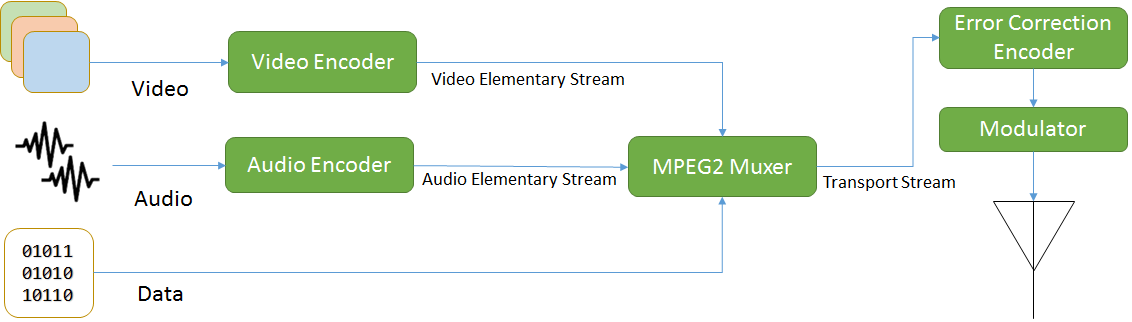
\includegraphics[width=1\linewidth]{figuras/diagrama_blocos_tvd.png}
\label{fig:diagrama_blocos_tvd}
\end{figure}
 
O Decreto presidencial número 8061, de 29 de julho de 2013, estabelece o cronograma de desligamento dos sistemas de transmissão de televisão analógica. Até 31 de dezembro de 2018, todos os transmissores analógicos devem ser desativados e os canais devem ser liberados. As outorgas serão revogadas e os canais devolvidos à união, que planeja utilizar a faixa dos 700MHz para implantar a tecnologia LTE, de telefonia móvel 4G, nesta faixa do espectro.

É portanto de grande interesse das emissoras de televisão atualizar seus transmissores para a tecnologia digital, para a manutenção da audiência. Se por um lado a nova tecnologia entrega melhor qualidade de vídeo e áudio ao telespectador, por outro lado a transmissão analógica deverá acabar e quem não se atualizar deverá cessar as transmissões. A televisão aberta digital representa para as emissoras uma grande oportunidade de concorrência com as operadoras de televisão paga, uma vez que a TV paga já é digitalizada há anos e sem essa oportunidade de transmissão, as emissoras perdiam a audiência dos usuários de televisores de alta definição para a TV paga.

Baseado no diagrama de blocos apresentado na \autoref{fig:diagrama_blocos_tvd}, é possível perceber que não basta atualizar apenas parte da cadeia de transmissão para a tecnologia digital a fim de entregar um produto de melhor qualidade ao telespectador. É necessário que os equipamentos de aquisição e manipulação sejam também atualizados para obter ganho efetivo de qualidade de imagem e áudio na recepção. Assim, é preciso considerar que a atualização de uma emissora de televisão requer um investimento considerável no projeto e aquisição dos equipamentos, bem como na implantação dos equipamentos.

Neste contexto de atualização do sistema de transmissão, a equipe de engenharia de projetos e implantação da RBS TV projetou e instalou as emissoras de televisão digital de 10 cidades no interior do Rio Grande do Sul e Santa Catarina durante o período de janeiro de 2013 até maio de 2014.

% ----------------------------------------------------------
% PARTE
% ----------------------------------------------------------
%\part{Preparação da pesquisa}
% ----------------------------------------------------------

% ---
% Capitulo com exemplos de comandos inseridos de arquivo externo 
% ---
%%% abtex2-modelo-include-comandos.tex, v-1.9.2 laurocesar
%% Copyright 2012-2014 by abnTeX2 group at http://abntex2.googlecode.com/ 
%%
%% This work may be distributed and/or modified under the
%% conditions of the LaTeX Project Public License, either version 1.3
%% of this license or (at your option) any later version.
%% The latest version of this license is in
%%   http://www.latex-project.org/lppl.txt
%% and version 1.3 or later is part of all distributions of LaTeX
%% version 2005/12/01 or later.
%%
%% This work has the LPPL maintenance status `maintained'.
%% 
%% The Current Maintainer of this work is the abnTeX2 team, led
%% by Lauro César Araujo. Further information are available on 
%% http://abntex2.googlecode.com/
%%
%% This work consists of the files abntex2-modelo-include-comandos.tex
%% and abntex2-modelo-img-marca.pdf
%%

% ---
% Este capítulo, utilizado por diferentes exemplos do abnTeX2, ilustra o uso de
% comandos do abnTeX2 e de LaTeX.
% ---
 
\chapter{Resultados de comandos}\label{cap_exemplos}

\chapterprecis{Isto é uma sinopse de capítulo. A ABNT não traz nenhuma
normatização a respeito desse tipo de resumo, que é mais comum em romances 
e livros técnicos.}\index{sinopse de capítulo}

% ---
\section{Codificação dos arquivos: UTF8}
% ---

A codificação de todos os arquivos do \abnTeX\ é \texttt{UTF8}. É necessário que
você utilize a mesma codificação nos documentos que escrever, inclusive nos
arquivos de base bibliográficas |.bib|.

% ---
\section{Citações diretas}
\label{sec-citacao}
% ---

\index{citações!diretas}Utilize o ambiente \texttt{citacao} para incluir
citações diretas com mais de três linhas:

\begin{citacao}
As citações diretas, no texto, com mais de três linhas, devem ser
destacadas com recuo de 4 cm da margem esquerda, com letra menor que a do texto
utilizado e sem as aspas. No caso de documentos datilografados, deve-se
observar apenas o recuo \cite[5.3]{NBR10520:2002}.
\end{citacao}

Use o ambiente assim:

\begin{verbatim}
\begin{citacao}
As citações diretas, no texto, com mais de três linhas [...] deve-se observar
apenas o recuo \cite[5.3]{NBR10520:2002}.
\end{citacao}
\end{verbatim}

O ambiente \texttt{citacao} pode receber como parâmetro opcional um nome de
idioma previamente carregado nas opções da classe (\autoref{sec-hifenizacao}). Nesse
caso, o texto da citação é automaticamente escrito em itálico e a hifenização é
ajustada para o idioma selecionado na opção do ambiente. Por exemplo:

\begin{verbatim}
\begin{citacao}[english]
Text in English language in italic with correct hyphenation.
\end{citacao}
\end{verbatim}

Tem como resultado:

\begin{citacao}[english]
Text in English language in italic with correct hyphenation.
\end{citacao}

\index{citações!simples}Citações simples, com até três linhas, devem ser
incluídas com aspas. Observe que em \LaTeX as aspas iniciais são diferentes das
finais: ``Amor é fogo que arde sem se ver''.

% ---
\section{Notas de rodapé}
% ---

As notas de rodapé são detalhadas pela NBR 14724:2011 na seção 5.2.1\footnote{As
notas devem ser digitadas ou datilografadas dentro das margens, ficando
separadas do texto por um espaço simples de entre as linhas e por filete de 5
cm, a partir da margem esquerda. Devem ser alinhadas, a partir da segunda linha
da mesma nota, abaixo da primeira letra da primeira palavra, de forma a destacar
o expoente, sem espaço entre elas e com fonte menor
\citeonline[5.2.1]{NBR14724:2011}.}\footnote{Caso uma série de notas sejam
criadas sequencialmente, o \abnTeX\ instrui o \LaTeX\ para que uma vírgula seja
colocada após cada número do expoente que indica a nota de rodapé no corpo do
texto.}\footnote{Verifique se os números do expoente possuem uma vírgula para
dividi-los no corpo do texto.}. 


% ---
\section{Tabelas}
% ---

\index{tabelas}A \autoref{tab-nivinv} é um exemplo de tabela construída em
\LaTeX.

\begin{table}[htb]
\ABNTEXfontereduzida
\caption[Níveis de investigação]{Níveis de investigação.}
\label{tab-nivinv}
\begin{tabular}{p{2.6cm}|p{6.0cm}|p{2.25cm}|p{3.40cm}}
  %\hline
   \textbf{Nível de Investigação} & \textbf{Insumos}  & \textbf{Sistemas de Investigação}  & \textbf{Produtos}  \\
    \hline
    Meta-nível & Filosofia\index{filosofia} da Ciência  & Epistemologia &
    Paradigma  \\
    \hline
    Nível do objeto & Paradigmas do metanível e evidências do nível inferior &
    Ciência  & Teorias e modelos \\
    \hline
    Nível inferior & Modelos e métodos do nível do objeto e problemas do nível inferior & Prática & Solução de problemas  \\
   % \hline
\end{tabular}
\legend{Fonte: \citeonline{van86}}
\end{table}

Já a \autoref{tabela-ibge} apresenta uma tabela criada conforme o padrão do
\citeonline{ibge1993} requerido pelas normas da ABNT para documentos técnicos e
acadêmicos.

\begin{table}[htb]
\IBGEtab{%
  \caption{Um Exemplo de tabela alinhada que pode ser longa
  ou curta, conforme padrão IBGE.}%
  \label{tabela-ibge}
}{%
  \begin{tabular}{ccc}
  \toprule
   Nome & Nascimento & Documento \\
  \midrule \midrule
   Maria da Silva & 11/11/1111 & 111.111.111-11 \\
  \midrule 
   João Souza & 11/11/2111 & 211.111.111-11 \\
  \midrule 
   Laura Vicuña & 05/04/1891 & 3111.111.111-11 \\
  \bottomrule
\end{tabular}%
}{%
  \fonte{Produzido pelos autores.}%
  \nota{Esta é uma nota, que diz que os dados são baseados na
  regressão linear.}%
  \nota[Anotações]{Uma anotação adicional, que pode ser seguida de várias
  outras.}%
  }
\end{table}


% ---
\section{Figuras}
% ---

\index{figuras}Figuras podem ser criadas diretamente em \LaTeX,
como o exemplo da \autoref{fig_circulo}.

\begin{figure}[htb]
	\caption{\label{fig_circulo}A delimitação do espaço}
	\begin{center}
	    \setlength{\unitlength}{5cm}
		\begin{picture}(1,1)
		\put(0,0){\line(0,1){1}}
		\put(0,0){\line(1,0){1}}
		\put(0,0){\line(1,1){1}}
		\put(0,0){\line(1,2){.5}}
		\put(0,0){\line(1,3){.3333}}
		\put(0,0){\line(1,4){.25}}
		\put(0,0){\line(1,5){.2}}
		\put(0,0){\line(1,6){.1667}}
		\put(0,0){\line(2,1){1}}
		\put(0,0){\line(2,3){.6667}}
		\put(0,0){\line(2,5){.4}}
		\put(0,0){\line(3,1){1}}
		\put(0,0){\line(3,2){1}}
		\put(0,0){\line(3,4){.75}}
		\put(0,0){\line(3,5){.6}}
		\put(0,0){\line(4,1){1}}
		\put(0,0){\line(4,3){1}}
		\put(0,0){\line(4,5){.8}}
		\put(0,0){\line(5,1){1}}
		\put(0,0){\line(5,2){1}}
		\put(0,0){\line(5,3){1}}
		\put(0,0){\line(5,4){1}}
		\put(0,0){\line(5,6){.8333}}
		\put(0,0){\line(6,1){1}}
		\put(0,0){\line(6,5){1}}
		\end{picture}
	\end{center}
	\legend{Fonte: os autores}
\end{figure}

Ou então figuras podem ser incorporadas de arquivos externos, como é o caso da
\autoref{fig_grafico}. Se a figura que ser incluída se tratar de um diagrama, um
gráfico ou uma ilustração que você mesmo produza, priorize o uso de imagens
vetoriais no formato PDF. Com isso, o tamanho do arquivo final do trabalho será
menor, e as imagens terão uma apresentação melhor, principalmente quando
impressas, uma vez que imagens vetorias são perfeitamente escaláveis para
qualquer dimensão. Nesse caso, se for utilizar o Microsoft Excel para produzir
gráficos, ou o Microsoft Word para produzir ilustrações, exporte-os como PDF e
os incorpore ao documento conforme o exemplo abaixo. No entanto, para manter a
coerência no uso de software livre (já que você está usando \LaTeX e \abnTeX),
teste a ferramenta \textsf{InkScape}\index{InkScape}
(\url{http://inkscape.org/}). Ela é uma excelente opção de código-livre para
produzir ilustrações vetoriais, similar ao CorelDraw\index{CorelDraw} ou ao Adobe
Illustrator\index{Adobe Illustrator}. De todo modo, caso não seja possível
utilizar arquivos de imagens como PDF, utilize qualquer outro formato, como
JPEG, GIF, BMP, etc. Nesse caso, você pode tentar aprimorar as imagens
incorporadas com o software livre \textsf{Gimp}\index{Gimp}
(\url{http://www.gimp.org/}). Ele é uma alternativa livre ao Adobe
Photoshop\index{Adobe Photoshop}.

\begin{figure}[htb]
	\caption{\label{fig_grafico}Gráfico produzido em Excel e salvo como PDF}
	\begin{center}
	    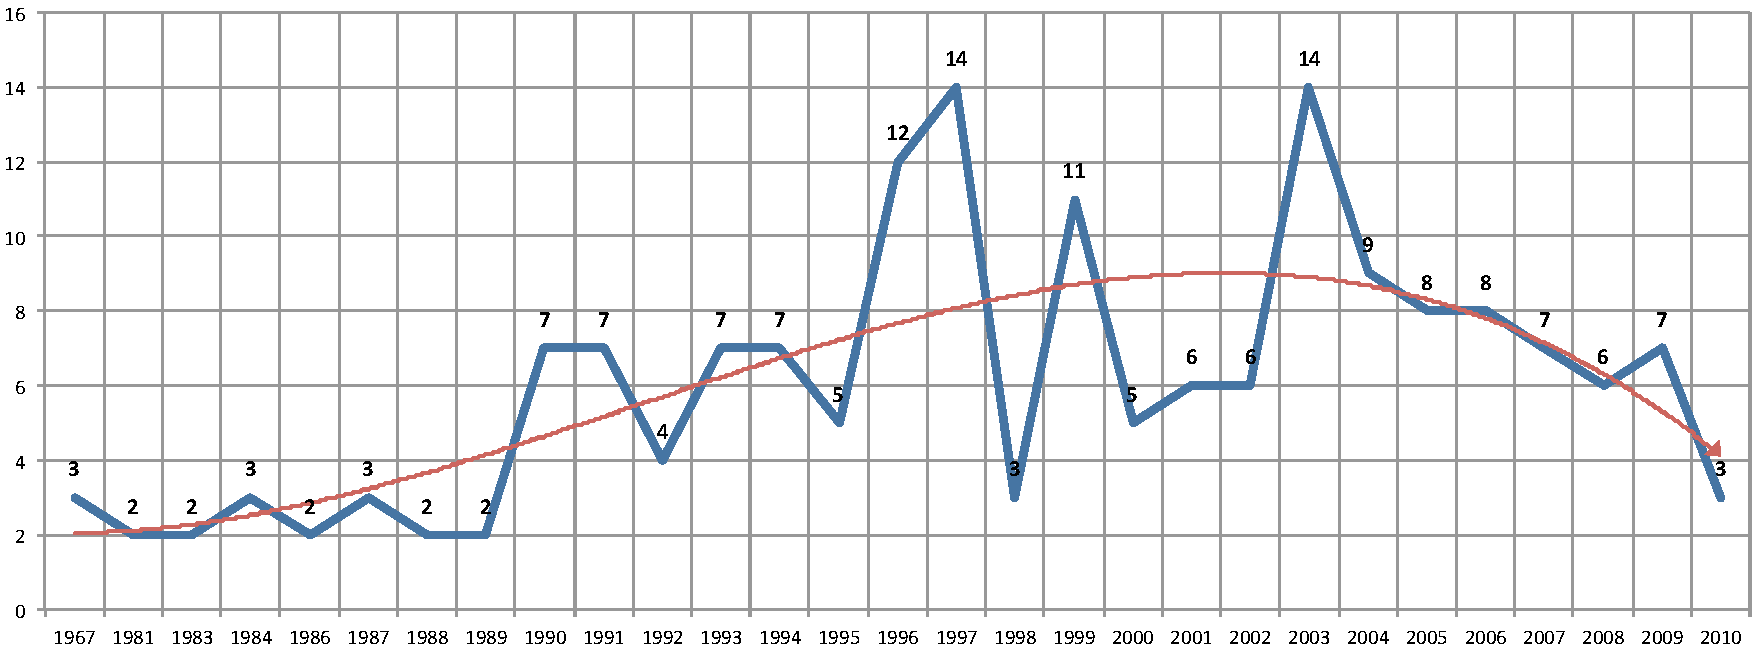
\includegraphics[scale=0.5]{abntex2-modelo-img-grafico.pdf}
	\end{center}
	\legend{Fonte: \citeonline[p. 24]{araujo2012}}
\end{figure}

% ---
\subsection{Figuras em \emph{minipages}}
% ---

\emph{Minipages} são usadas para inserir textos ou outros elementos em quadros
com tamanhos e posições controladas. Veja o exemplo da
\autoref{fig_minipage_imagem1} e da \autoref{fig_minipage_grafico2}.

\begin{figure}[htb]
 \label{teste}
 \centering
  \begin{minipage}{0.4\textwidth}
    \centering
    \caption{Imagem 1 da minipage} \label{fig_minipage_imagem1}
    
\includegraphics[scale=0.9]{abntex2-modelo-img-marca.pdf}
    \legend{Fonte: Produzido pelos autores}
  \end{minipage}
  \hfill
  \begin{minipage}{0.4\textwidth}
    \centering
    \caption{Grafico 2 da minipage} \label{fig_minipage_grafico2}
    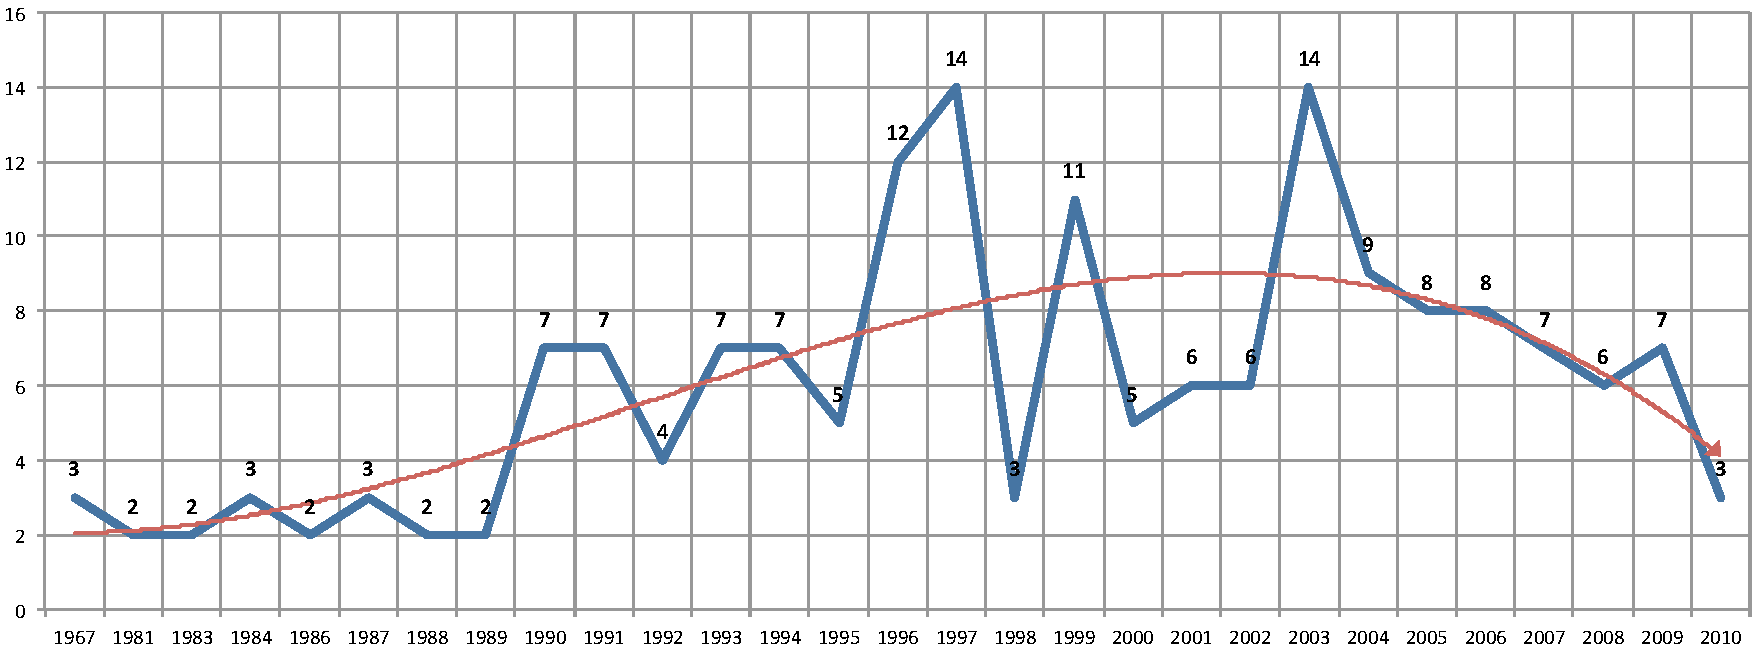
\includegraphics[scale=0.2]{abntex2-modelo-img-grafico.pdf}
    \legend{Fonte: \citeonline[p. 24]{araujo2012}}
  \end{minipage}
\end{figure}

Observe que, segundo a \citeonline[seções 4.2.1.10 e 5.8]{NBR14724:2011}, as
ilustrações devem sempre ter numeração contínua e única em todo o documento:

\begin{citacao}
Qualquer que seja o tipo de ilustração, sua identificação aparece na parte
superior, precedida da palavra designativa (desenho, esquema, fluxograma,
fotografia, gráfico, mapa, organograma, planta, quadro, retrato, figura,
imagem, entre outros), seguida de seu número de ordem de ocorrência no texto,
em algarismos arábicos, travessão e do respectivo título. Após a ilustração, na
parte inferior, indicar a fonte consultada (elemento obrigatório, mesmo que
seja produção do próprio autor), legenda, notas e outras informações
necessárias à sua compreensão (se houver). A ilustração deve ser citada no
texto e inserida o mais próximo possível do trecho a que se
refere. \cite[seções 5.8]{NBR14724:2011}
\end{citacao}

% ---
\section{Expressões matemáticas}
% ---

\index{expressões matemáticas}Use o ambiente \texttt{equation} para escrever
expressões matemáticas numeradas:

\begin{equation}
  \forall x \in X, \quad \exists \: y \leq \epsilon
\end{equation}

Escreva expressões matemáticas entre \$ e \$, como em $ \lim_{x \to \infty}
\exp(-x) = 0 $, para que fiquem na mesma linha.

Também é possível usar colchetes para indicar o início de uma expressão
matemática que não é numerada.

\[
\left|\sum_{i=1}^n a_ib_i\right|
\le
\left(\sum_{i=1}^n a_i^2\right)^{1/2}
\left(\sum_{i=1}^n b_i^2\right)^{1/2}
\]

Consulte mais informações sobre expressões matemáticas em
\url{https://code.google.com/p/abntex2/wiki/Referencias}.

% ---
\section{Enumerações: alíneas e subalíneas}
% ---

\index{alíneas}\index{subalíneas}\index{incisos}Quando for necessário enumerar
os diversos assuntos de uma seção que não possua título, esta deve ser
subdividida em alíneas \cite[4.2]{NBR6024:2012}:

\begin{alineas}

  \item os diversos assuntos que não possuam título próprio, dentro de uma mesma
  seção, devem ser subdivididos em alíneas; 
  
  \item o texto que antecede as alíneas termina em dois pontos;
  \item as alíneas devem ser indicadas alfabeticamente, em letra minúscula,
  seguida de parêntese. Utilizam-se letras dobradas, quando esgotadas as
  letras do alfabeto;

  \item as letras indicativas das alíneas devem apresentar recuo em relação à
  margem esquerda;

  \item o texto da alínea deve começar por letra minúscula e terminar em
  ponto-e-vírgula, exceto a última alínea que termina em ponto final;

  \item o texto da alínea deve terminar em dois pontos, se houver subalínea;

  \item a segunda e as seguintes linhas do texto da alínea começa sob a
  primeira letra do texto da própria alínea;
  
  \item subalíneas \cite[4.3]{NBR6024:2012} devem ser conforme as alíneas a
  seguir:

  \begin{alineas}
     \item as subalíneas devem começar por travessão seguido de espaço;

     \item as subalíneas devem apresentar recuo em relação à alínea;

     \item o texto da subalínea deve começar por letra minúscula e terminar em
     ponto-e-vírgula. A última subalínea deve terminar em ponto final, se não
     houver alínea subsequente;

     \item a segunda e as seguintes linhas do texto da subalínea começam sob a
     primeira letra do texto da própria subalínea.
  \end{alineas}
  
  \item no \abnTeX\ estão disponíveis os ambientes \texttt{incisos} e
  \texttt{subalineas}, que em suma são o mesmo que se criar outro nível de
  \texttt{alineas}, como nos exemplos à seguir:
  
  \begin{incisos}
    \item \textit{Um novo inciso em itálico};
  \end{incisos}
  
  \item Alínea em \textbf{negrito}:
  
  \begin{subalineas}
    \item \textit{Uma subalínea em itálico};
    \item \underline{\textit{Uma subalínea em itálico e sublinhado}}; 
  \end{subalineas}
  
  \item Última alínea com \emph{ênfase}.
  
\end{alineas}

% ---
\section{Espaçamento entre parágrafos e linhas}
% ---

\index{espaçamento!dos parágrafos}O tamanho do parágrafo, espaço entre a margem
e o início da frase do parágrafo, é definido por:

\begin{verbatim}
   \setlength{\parindent}{1.3cm}
\end{verbatim}

\index{espaçamento!do primeiro parágrafo}Por padrão, não há espaçamento no
primeiro parágrafo de cada início de divisão do documento
(\autoref{sec-divisoes}). Porém, você pode definir que o primeiro parágrafo
também seja indentado, como é o caso deste documento. Para isso, apenas inclua o
pacote \textsf{indentfirst} no preâmbulo do documento:

\begin{verbatim}
   \usepackage{indentfirst}      % Indenta o primeiro parágrafo de cada seção.
\end{verbatim}

\index{espaçamento!entre os parágrafos}O espaçamento entre um parágrafo e outro
pode ser controlado por meio do comando:

\begin{verbatim}
  \setlength{\parskip}{0.2cm}  % tente também \onelineskip
\end{verbatim}

\index{espaçamento!entre as linhas}O controle do espaçamento entre linhas é
definido por:

\begin{verbatim}
  \OnehalfSpacing       % espaçamento um e meio (padrão); 
  \DoubleSpacing        % espaçamento duplo
  \SingleSpacing        % espaçamento simples	
\end{verbatim}

Para isso, também estão disponíveis os ambientes:

\begin{verbatim}
  \begin{SingleSpace} ...\end{SingleSpace}
  \begin{Spacing}{hfactori} ... \end{Spacing}
  \begin{OnehalfSpace} ... \end{OnehalfSpace}
  \begin{OnehalfSpace*} ... \end{OnehalfSpace*}
  \begin{DoubleSpace} ... \end{DoubleSpace}
  \begin{DoubleSpace*} ... \end{DoubleSpace*} 
\end{verbatim}

Para mais informações, consulte \citeonline[p. 47-52 e 135]{memoir}.

% ---
\section{Inclusão de outros arquivos}\label{sec-include}
% ---

É uma boa prática dividir o seu documento em diversos arquivos, e não
apenas escrever tudo em um único. Esse recurso foi utilizado neste
documento. Para incluir diferentes arquivos em um arquivo principal,
de modo que cada arquivo incluído fique em uma página diferente, utilize o
comando:

\begin{verbatim}
   \include{documento-a-ser-incluido}      % sem a extensão .tex
\end{verbatim}

Para incluir documentos sem quebra de páginas, utilize:

\begin{verbatim}
   \input{documento-a-ser-incluido}      % sem a extensão .tex
\end{verbatim}

% ---
\section{Compilar o documento \LaTeX}
% ---

Geralmente os editores \LaTeX, como o
TeXlipse\footnote{\url{http://texlipse.sourceforge.net/}}, o
Texmaker\footnote{\url{http://www.xm1math.net/texmaker/}}, entre outros,
compilam os documentos automaticamente, de modo que você não precisa se
preocupar com isso.

No entanto, você pode compilar os documentos \LaTeX usando os seguintes
comandos, que devem ser digitados no \emph{Prompt de Comandos} do Windows ou no
\emph{Terminal} do Mac ou do Linux:

\begin{verbatim}
   pdflatex ARQUIVO_PRINCIPAL.tex
   bibtex ARQUIVO_PRINCIPAL.aux
   makeindex ARQUIVO_PRINCIPAL.idx 
   makeindex ARQUIVO_PRINCIPAL.nlo -s nomencl.ist -o ARQUIVO_PRINCIPAL.nls
   pdflatex ARQUIVO_PRINCIPAL.tex
   pdflatex ARQUIVO_PRINCIPAL.tex
\end{verbatim}

% ---
\section{Remissões internas}
% ---

Ao nomear a \autoref{tab-nivinv} e a \autoref{fig_circulo}, apresentamos um
exemplo de remissão interna, que também pode ser feita quando indicamos o
\autoref{cap_exemplos}, que tem o nome \emph{\nameref{cap_exemplos}}. O número
do capítulo indicado é \ref{cap_exemplos}, que se inicia à
\autopageref{cap_exemplos}\footnote{O número da página de uma remissão pode ser
obtida também assim:
\pageref{cap_exemplos}.}.
Veja a \autoref{sec-divisoes} para outros exemplos de remissões internas entre
seções, subseções e subsubseções.

O código usado para produzir o texto desta seção é:

\begin{verbatim}
Ao nomear a \autoref{tab-nivinv} e a \autoref{fig_circulo}, apresentamos um
exemplo de remissão interna, que também pode ser feita quando indicamos o
\autoref{cap_exemplos}, que tem o nome \emph{\nameref{cap_exemplos}}. O número
do capítulo indicado é \ref{cap_exemplos}, que se inicia à
\autopageref{cap_exemplos}\footnote{O número da página de uma remissão pode ser
obtida também assim:
\pageref{cap_exemplos}.}.
Veja a \autoref{sec-divisoes} para outros exemplos de remissões internas entre
seções, subseções e subsubseções.
\end{verbatim}

% ---
\section{Divisões do documento: seção}\label{sec-divisoes}
% ---

Esta seção testa o uso de divisões de documentos. Esta é a
\autoref{sec-divisoes}. Veja a \autoref{sec-divisoes-subsection}.

\subsection{Divisões do documento: subseção}\label{sec-divisoes-subsection}

Isto é uma subseção. Veja a \autoref{sec-divisoes-subsubsection}, que é uma
\texttt{subsubsection} do \LaTeX, mas é impressa chamada de ``subseção'' porque
no Português não temos a palavra ``subsubseção''.

\subsubsection{Divisões do documento: subsubseção}
\label{sec-divisoes-subsubsection}

Isto é uma subsubseção.

\subsubsection{Divisões do documento: subsubseção}

Isto é outra subsubseção.

\subsection{Divisões do documento: subseção}\label{sec-exemplo-subsec}

Isto é uma subseção.

\subsubsection{Divisões do documento: subsubseção}

Isto é mais uma subsubseção da \autoref{sec-exemplo-subsec}.


\subsubsubsection{Esta é uma subseção de quinto
nível}\label{sec-exemplo-subsubsubsection}

Esta é uma seção de quinto nível. Ela é produzida com o seguinte comando:

\begin{verbatim}
\subsubsubsection{Esta é uma subseção de quinto
nível}\label{sec-exemplo-subsubsubsection}
\end{verbatim}

\subsubsubsection{Esta é outra subseção de quinto nível}\label{sec-exemplo-subsubsubsection-outro}

Esta é outra seção de quinto nível.


\paragraph{Este é um parágrafo numerado}\label{sec-exemplo-paragrafo}

Este é um exemplo de parágrafo nomeado. Ele é produzida com o comando de
parágrafo:

\begin{verbatim}
\paragraph{Este é um parágrafo nomeado}\label{sec-exemplo-paragrafo}
\end{verbatim}

A numeração entre parágrafos numeradaos e subsubsubseções são contínuas.

\paragraph{Esta é outro parágrafo numerado}\label{sec-exemplo-paragrafo-outro}

Esta é outro parágrafo nomeado.

% ---
\section{Este é um exemplo de nome de seção longo. Ele deve estar
alinhado à esquerda e a segunda e demais linhas devem iniciar logo abaixo da
primeira palavra da primeira linha}
% ---

Isso atende à norma \citeonline[seções de 5.2.2 a 5.2.4]{NBR14724:2011} 
 e \citeonline[seções de 3.1 a 3.8]{NBR6024:2012}.

% ---
\section{Diferentes idiomas e hifenizações}
\label{sec-hifenizacao}
% ---

Para usar hifenizações de diferentes idiomas, inclua nas opções do documento o
nome dos idiomas que o seu texto contém. Por exemplo (para melhor
visualização, as opções foram quebras em diferentes linhas):

\begin{verbatim}
\documentclass[
	12pt,
	openright,
	twoside,
	a4paper,
	english,
	french,
	spanish,
	brazil
	]{abntex2}
\end{verbatim}

O idioma português-brasileiro (\texttt{brazil}) é incluído automaticamente pela
classe \textsf{abntex2}. Porém, mesmo assim a opção \texttt{brazil} deve ser
informada como a última opção da classe para que todos os pacotes reconheçam o
idioma. Vale ressaltar que a última opção de idioma é a utilizada por padrão no
documento. Desse modo, caso deseje escrever um texto em inglês que tenha
citações em português e em francês, você deveria usar o preâmbulo como abaixo:

\begin{verbatim}
\documentclass[
	12pt,
	openright,
	twoside,
	a4paper,
	french,
	brazil,
	english
	]{abntex2}
\end{verbatim}

A lista completa de idiomas suportados, bem como outras opções de hifenização,
estão disponíveis em \citeonline[p.~5-6]{babel}.

Exemplo de hifenização em inglês\footnote{Extraído de:
\url{http://en.wikibooks.org/wiki/LaTeX/Internationalization}}:

\begin{otherlanguage*}{english}
\textit{Text in English language. This environment switches all language-related
definitions, like the language specific names for figures, tables etc. to the other
language. The starred version of this environment typesets the main text
according to the rules of the other language, but keeps the language specific
string for ancillary things like figures, in the main language of the document.
The environment hyphenrules switches only the hyphenation patterns used; it can
also be used to disallow hyphenation by using the language name
`nohyphenation'.}
\end{otherlanguage*}

Exemplo de hifenização em francês\footnote{Extraído de:
\url{http://bigbrowser.blog.lemonde.fr/2013/02/17/tu-ne-tweeteras-point-le-vatican-interdit-aux-cardinaux-de-tweeter-pendant-le-conclave/}}:

\begin{otherlanguage*}{french}
\textit{Texte en français. Pas question que Twitter ne vienne faire une
concurrence déloyale à la traditionnelle fumée blanche qui marque l'élection
d'un nouveau pape. Pour éviter toute fuite précoce, le Vatican a donc pris un
peu d'avance, et a déjà interdit aux cardinaux qui prendront part au vote
d'utiliser le réseau social, selon Catholic News Service. Une mesure valable
surtout pour les neuf cardinaux – sur les 117 du conclave – pratiquants très
actifs de Twitter, qui auront interdiction pendant toute la période de se
connecter à leur compte.}
\end{otherlanguage*}

Pequeno texto em espanhol\footnote{Extraído de:
\url{http://internacional.elpais.com/internacional/2013/02/17/actualidad/1361102009_913423.html}}:

\foreignlanguage{spanish}{\textit{Decenas de miles de personas ovacionan al pontífice en su
penúltimo ángelus dominical, el primero desde que anunciase su renuncia. El Papa se
centra en la crítica al materialismo}}.

O idioma geral do texto por ser alterado como no exemplo seguinte:

\begin{verbatim}
  \selectlanguage{english}
\end{verbatim}

Isso altera automaticamente a hifenização e todos os nomes constantes de
referências do documento para o idioma inglês. Consulte o manual da classe
\cite{abntex2classe} para obter orientações adicionais sobre internacionalização de
documentos produzidos com \abnTeX.

A \autoref{sec-citacao} descreve o ambiente \texttt{citacao} que pode receber
como parâmetro um idioma a ser usado na citação.

% ---
\section{Consulte o manual da classe \textsf{abntex2}}
% ---

Consulte o manual da classe \textsf{abntex2} \cite{abntex2classe} para uma
referência completa das macros e ambientes disponíveis. 

Além disso, o manual possui informações adicionais sobre as normas ABNT
observadas pelo \abnTeX\ e considerações sobre eventuais requisitos específicos
não atendidos, como o caso da \citeonline[seção 5.2.2]{NBR14724:2011}, que
especifica o espaçamento entre os capítulos e o início do texto, regra
propositalmente não atendida pelo presente modelo.

% ---
\section{Referências bibliográficas}
% ---

A formatação das referências bibliográficas conforme as regras da ABNT são um
dos principais objetivos do \abnTeX. Consulte os manuais
\citeonline{abntex2cite} e \citeonline{abntex2cite-alf} para obter informações
sobre como utilizar as referências bibliográficas.

%-
\subsection{Acentuação de referências bibliográficas}
%-

Normalmente não há problemas em usar caracteres acentuados em arquivos
bibliográficos (\texttt{*.bib}). Porém, como as regras da ABNT fazem uso quase
abusivo da conversão para letras maiúsculas, é preciso observar o modo como se
escreve os nomes dos autores. Na ~\autoref{tabela-acentos} você encontra alguns
exemplos das conversões mais importantes. Preste atenção especial para `ç' e `í'
que devem estar envoltos em chaves. A regra geral é sempre usar a acentuação
neste modo quando houver conversão para letras maiúsculas.

\begin{table}[htbp]
\caption{Tabela de conversão de acentuação.}
\label{tabela-acentos}

\begin{center}
\begin{tabular}{ll}\hline\hline
acento & \textsf{bibtex}\\
à á ã & \verb+\`a+ \verb+\'a+ \verb+\~a+\\
í & \verb+{\'\i}+\\
ç & \verb+{\c c}+\\
\hline\hline
\end{tabular}
\end{center}
\end{table}


% ---
\section{Precisa de ajuda?}
% ---

Consulte a FAQ com perguntas frequentes e comuns no portal do \abnTeX:
\url{https://code.google.com/p/abntex2/wiki/FAQ}.

Inscreva-se no grupo de usuários \LaTeX:
\url{http://groups.google.com/group/latex-br}, tire suas dúvidas e ajude
outros usuários.

Participe também do grupo de desenvolvedores do \abnTeX:
\url{http://groups.google.com/group/abntex2} e faça sua contribuição à
ferramenta.

% ---
\section{Você pode ajudar?}
% ---

Sua contribuição é muito importante! Você pode ajudar na divulgação, no
desenvolvimento e de várias outras formas. Veja como contribuir com o \abnTeX\
em \url{https://code.google.com/p/abntex2/wiki/ComoContribuir}.

% ---
\section{Quer customizar os modelos do \abnTeX\ para sua instituição ou
universidade?}
% ---

Veja como customizar o \abnTeX\ em:
\url{https://code.google.com/p/abntex2/wiki/ComoCustomizar}.


% ---

% ----------------------------------------------------------
% PARTE
% ----------------------------------------------------------
%\part{Referenciais teóricos}
% ----------------------------------------------------------

% ---
% Capitulo de revisão de literatura
% ---
\section{Apresentação da Empresa e do Estágio}

A RBS TV é uma emissora de televisão afiliada da Rede Globo, com atuação nos estados do Rio Grande do Sul e Santa Catarina, na região sul do Brasil. Além de retransmitir a programação da Rede Globo na maior parte do tempo, também exibe produções próprias diariamente, nos segmentos informativos e de entretenimento.

Para garantir a ampliação e a manutenção de sua infraestrutura, a empresa tem uma grande equipe técnica que atua projetando a implantação de novas tecnologias e prestando suporte à infraestrutura existente. O setor técnico é composto de engenheiros e técnicos formados em assuntos associados a televisão, como Engenharia Elétrica, Engenharia de Telecomunicações, Engenharia de Computação, Técnico em Eletrônica e Técnico em Telecomunicação.

A equipe da engenharia de projetos tem como objetivo projetar e implantar soluções que agreguem as inovações tecnológicas atuais ao fluxo de trabalho das equipes de jornalismo e produção.

\section{Apresentação do Projeto}

O projeto específico em que o estágio ocorreu consiste em projetar e instalar geradoras de televisão em dez cidades com mais de 50 mil habitantes do interior do Rio Grande do Sul e Santa Catarina. São elas Santa Cruz do Sul, Bagé, Uruguaiana, Rio Grande, Erechim e Cruz Alta e Santa Rosa no Rio Grande do Sul, e Criciúma, Chapecó e Joaçaba, em Santa Catarina.

São tarefas da equipe o projeto técnico e a escolha dos equipamentos utilizados nas instalações. Optou-se por criar um padrão de emissora que foi replicado para todas as dez geradoras, visando minimizar o retrabalho de projeto e facilitar a atuação da equipe de suporte, uma vez que com um projeto padrão os equipamentos são iguais em todas as sedes.

A equipe é dividida em duas áreas: gestão e implantação. A área de gestão é responsável pela interface com outros setores internos da empresa, como comercial, suprimentos, logística, financeiro; bem como fornecedores externos de produtos e serviços. A área de implantação é responsável pelo projeto técnico, bem como por visitar as emissoras, executar a instalação dos equipamentos e supervisionar a atuação dos terceiros que atuam lá.

\section{Descrição das tarefas executadas}

As atividades do estágio foram desenvolvidas na sede da empresa, em Porto Alegre, vinculadas tanto à equipe de gestão quanto à equipe de implantação. O estagiário constituiu a interface entre as duas áreas, dando suporte à equipe que estava em constantes visitas ao interior para assegurar que o projeto seria executado corretamente.

As principais tarefas exercidas durante o estágio foram:

\begin{itemize}

\item parametrização e configuração dos equipamentos, a fim de respeitar as normas brasileiras e o padrão de qualidade de transmissão objetivado pela empresa;

\item coordenação do envio e recebimento dos equipamentos para as dez geradoras, programando datas de coletas e entregas dos equipamentos de Porto Alegre para as geradoras;

\item elaboração de documentos técnicos tutoriais para instruir os técnicos locais e os operadores sobre o funcionamento dos equipamentos;

\item elaboração de diagramas unifilares do fluxo de sinal de vídeo, áudio e dados ao longo da cadeia de transmissão

\item elaboração de modelos em três dimensões dos ambientes envolvidos nas geradoras, a fim de prever possíveis limitações de espaço e visando otimizar o espaço dos ambientes, prezando pela ergonomia dos operadores;

\item avaliação técnica de soluções disponíveis no mercado para problemas que ainda não tinham sido solucionados pela equipe, como o isolamento e a monitoração da conexão com terceirizados;
\end{itemize}

\chapter{Desenvolvimento}

\section{Diagramas de fluxo de sinal}

A documentação é fundamental para a manutenção de qualquer infraestrutura. Sem um diagrama atualizado, é praticamente impossível manter o sistema funcionando corretamente sem depender de alguém que conheça todo o sistema de memória. Assim, foram confeccionados diagramas unifilares em Microsoft Visio de cada parte do sistema. Os diagramas são confidenciais e não puderam ser replicados no relatório.

\section{Modelos em três dimensões}

Os desenhos em três dimensões dos ambientes técnicos e de operações possibilitaram prever os caminhos por onde passariam os cabos de alimentação elétrica, os cabos de vídeo e de áudio, bem como os cabos de rede e de controle, e também as eletrocalhas utilizadas para conduzir os cabos. Também assim, previu-se as reformas civis, de construção e demolição de paredes para reorganizar os ambientes.

Com estes desenhos preliminares, foi possível estimar o consumo de cabos para cada instalação e também prever caminhos críticos por onde haveria dificuldade de transpor determinados obstáculos, como vigas que deveriam ser contornadas ou sobreposição de calhas na chegada aos racks de equipamentos. Os desenhos visaram otimizar os aspectos ergonômicos de trabalho e a funcionalidade dos ambientes, economizar materiais e minimizar o retrabalho futuro.

O software escolhido para realizar os desenhos é o Google Sketchup. A seguir é apresentado um exemplo de utilização do software para prever o caminho de uma eletrocalha desviando de uma viga. Na \autoref{fig:real_sketchup_desenho} vê-se o desenho previamente realizado e na \autoref{fig:real_sketchup} vê-se o que de fato foi executado.

\begin{figure}[!h]
\centering
\caption{Desenho do projeto em 3D do ambiente.}
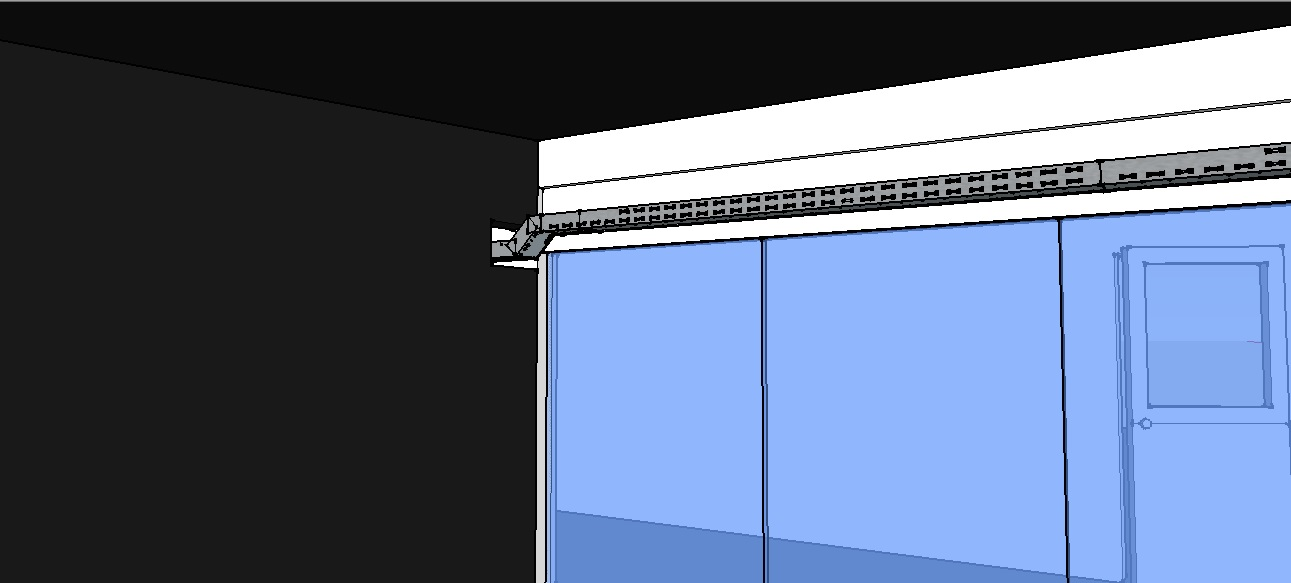
\includegraphics[width=0.8\linewidth]{figuras/real_sketchup_desenho.jpg}
\\Fonte: O autor.
\label{fig:real_sketchup_desenho}
\end{figure}

\begin{figure}[!h]
\centering
\caption{Foto real do ambiente projetado.}
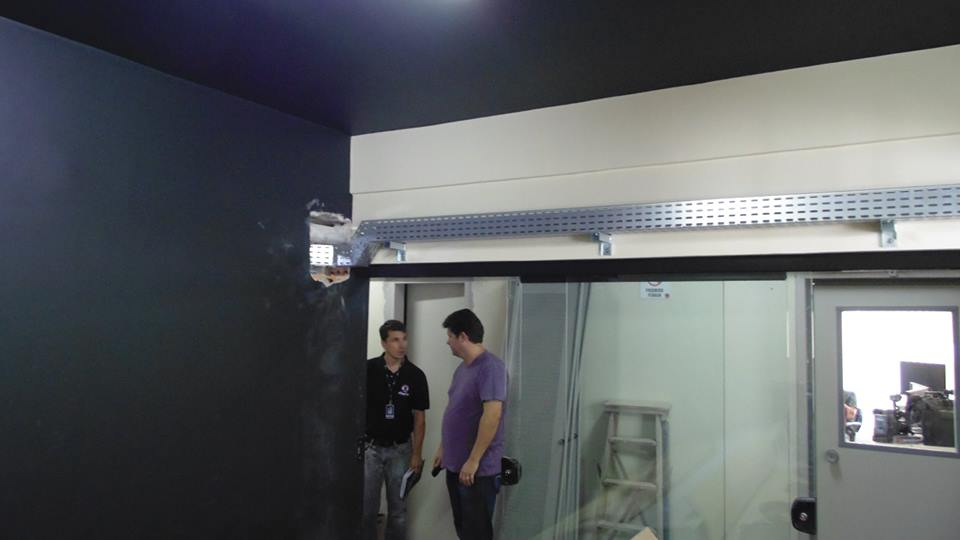
\includegraphics[width=0.8\linewidth]{figuras/real_sketchup.jpg}
\\Fonte: Reprodução RBSTV.
\label{fig:real_sketchup}
\end{figure}

\section{Descritivo de Equipamentos}

Na instalação padrão de uma emissora de televisão são necessários uma centena de equipamentos para exibição do conteúdo, monitoração, seleção das fontes de sinal, comutação automática em caso de falha e controle dos periféricos. Seria inviável descrever todos os equipamentos neste relatório suscinto, então optou-se por abordar aspectos cruciais para o funcionamento em alguns breves parágrafos.

\subsection{Sinais de Referência}

Para garantir o correto funcionamento dos equipamentos em conjunto é indispensável utilizar um sinal que garanta o sincronismo entre todos eles. Este sinal funciona como se fosse um sinal de \textit{clock} global do sistema. O sinal utilizado na instalação é um sinal de Black Burst de vídeo analógico, que é basicamente um pulso de sinal com taxa de repetição constante e forma de onda conhecida, de modo que é ideal para servir de sinal de sincronismo.

O equipamento responsável por gerar este sinal é o Pulse Generator PG8000 da Tektronix. Além do sinal de Black Burst para sincronismo, ele também pode gerar sinais de vídeo em padrões analógicos e digitais, para testes de transmissão, como tons de áudio de frequências definidas ou quadros de vido estáticos com barras coloridas.

\subsection{Redundância}

A redundância na geração dos sinais é indispensável para se garantir um tempo médio entre falhas baixo. A RBS TV assume com a Rede Globo contratos que exigem um tempo máximo de falhas, e cada falha deve ser reportada à emissora.

Nessas condições, optou-se por projetar um sistema com dois caminhos independentes de sinal, desde as fontes de vídeo e áudio até os transmissores. O objetivo é prevenir-se de eventuais falhas nos equipamentos e minimizar o tempo fora de serviço.

Um dos equipamentos responsáveis é o Automatic ChangeOver ACO6800+ISCST da Imagine Communications\cite{harris}, cujo diagrama de blocos interno pode ser visto na \autoref{fig:aco_block_diag}.

\begin{figure}[!h]
\centering
\caption{Diagrama de blocos do ACO6800+ISCST.}
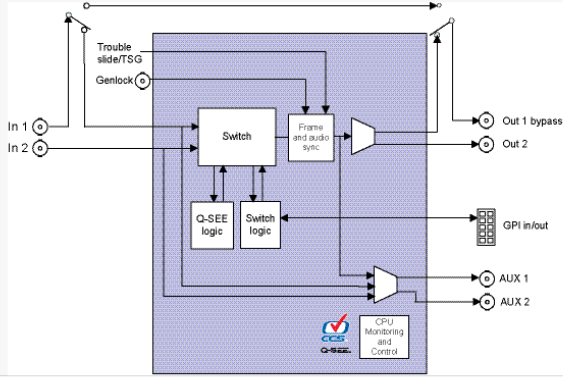
\includegraphics[width=0.5\linewidth]{figuras/aco_block_diag.png}
\\Fonte: O autor.
\label{fig:aco_block_diag}
\end{figure}

Vê-se na figura a presença de dois relés mecânicos, responsáveis por, em caso de pane no dispositivo, efetuar o \textit{bypass} do sinal de maneira física. Quando estiver em operação normal, o ACO envia o sinal da entrada In1 para as saídas Out1 e Out2, enquanto monitora o sinal de vídeo da entrada In1. Em caso de falha no sinal, ele comuta automaticamente as saídas para a entrada In2.

O equipamento conta com uma série de configurações possíveis para operação automática: é possível, por exemplo escolher os tipos de falha de vídeo que devem ser usados como gatilho para a comutação, bem como o tempo que se deve esperar para comutar. Ainda pode-se optar por fazer uma comutação manual utilizando um painel acessório através do conector GPI(General Purpose Interface).

É interessante notar, ainda, que o equipamento dispõe de uma entrada de sinal de referência, ou \textit{Genlock}, pois é preciso que a comutação seja feita de maneira sincronizada com a mudança de um quadro de vídeo para o próximo, para evitar que haja variações na imagem.

\section{Medições de qualidade de sinal digital}

O diagrama de olho permite avaliar a qualidade do sinal analógico, da camada física, que transporta o sinal digital. O jitter é uma medida da variação do atraso relativo entre os sinais de vídeo, causado basicamente por problemas com cabos de má qualidade, muito extensos ou com falhas, como dobras acentuadas ou rompimento da malha.

O ruído é causado pela indução magnética dos equipamentos ao redor do cabo. Caso ele tenha uma malha de proteção fina, pode deixar o condutor de sinal exposto a induções de sinais externos ao que se deseja transportar, originando ruido.

A seguir são apresentadas duas imagens com diagramas de olho. Na \autoref{fig:olho_pouco_jitter} há pouco jitter e pouco ruido e na \autoref{fig:olho_muito_jitter} há consideravelmente bastante jitter e ruido. Um nível alto de jitter pode levar o receptor a não diferenciar os instantes de mudança de um valor binário para o outro, enquanto que o ruído interfere nos níveis de sinal para cada valor lógico.

\begin{figure}[!h]
\centering
\caption{Diagrama de olho com pouco jitter e ruido.}
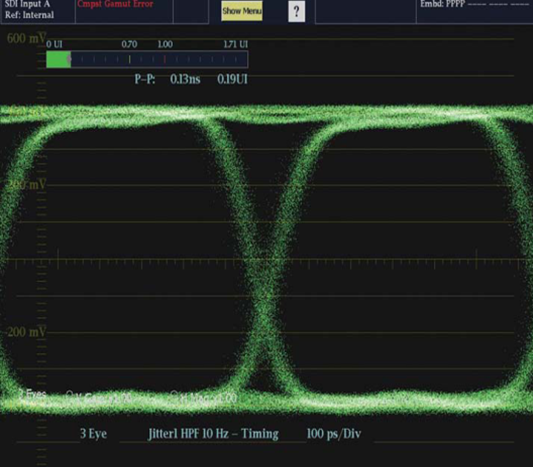
\includegraphics[width=0.5\linewidth]{figuras/olho_pouco_jitter.png}
\\Fonte: Tektronix.
\label{fig:olho_pouco_jitter}
\end{figure}

\begin{figure}[!h]
\centering
\caption{Diagrama de olho com muito jitter e ruido.}
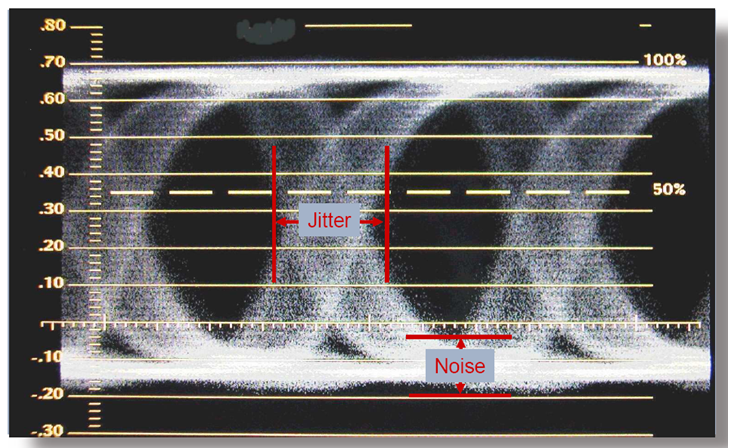
\includegraphics[width=0.5\linewidth]{figuras/olho_muito_jitter.png}
\\Fonte: Tektronix.
\label{fig:olho_muito_jitter}
\end{figure}

% ---
% Conclusão (outro exemplo de capítulo sem numeração e presente no sumário)
% ---
\chapter[Conclusões]{Conclusões}
%\addcontentsline{toc}{chapter}{Conclusions and Future Development}
% ---

O local de trabalho é muito bom em termos de aprendizado técnico e prático dos afazeres de uma equipe de projetos. Com experiência em gestão de projetos, o gerente foi responsável e buscou realizar reuniões diárias nos primeiros meses de estágio para garantir a ambientação do estagiário na equipe.

O objetivo de desenvolvimento pessoal foi atingido satisfatoriamente, com aquisição de capacidades técnicas específicas que não se tem a oportunidade de desenvolver na UFRGS por falta de disciplinas específicas sobre televisão analógica e digital. Foi possível aprender como é o fluxo de sinal desde a captação, passando pelo armazenamento em diferentes mídias, depois sendo codificado e sendo finalmente transmitido nos padrões analógico e digital.

Foi possível também compreender as condições políticas e contratuais que interferem nos aspectos técnicos e de planejamento, como a necessidade de redundância de toda a cadeia de transmissão para minimizar os tempos de falha.

É também clara a utilidade do planejamento do layout dos ambientes para prever dificuldades e evitar retrabalhos após a instalação, seja pela possibilidade de identificar obstáculos físicos, seja por prever a posição específica dos operadores considerando aspectos ergonômicos da posição de trabalho. Com isso, pode-se até evitar eventuais lesões dos operadores.

A equipe é preocupada em integrar o estagiário nos diferentes núcleos envolvidos na gestão do projeto. É possível ao estagiário interagir com as equipes de suprimentos, logística e financeira, além de participar ativamente do projeto técnico evidentemente. Com isso, ainda que o estagiário não tenha conhecimentos específicos logo que ingressa na vaga, ele pode participar de outros procedimentos inerentes à gestão de um projeto, mas que não se aprende nas disciplinas teóricas do curso.

% ----------------------------------------------------------
% ELEMENTOS PÓS-TEXTUAIS
% ----------------------------------------------------------
\postextual
% ----------------------------------------------------------

% ----------------------------------------------------------
% Referências bibliográficas
% ----------------------------------------------------------
\bibliography{relatorio_estagio.bib}

\end{document}
